\documentclass[a4paper, 12pt]{ppgeb}

% |--- Títulos, autor, banca ---|----------------------{{{
% Autor:
% Substituta  as informações nos comandos a seguir, até a linha começando
% com \membrobancaexterno.
% Em \title: título na forma principal, como aparecerá em algumas páginas
% Em \tituloficha: título como aparecerá na ficha catalográfica; idêntico
% ao anterior, mas com possíveis quebras manuais de linha (usar \\ quando
% necessário, para ajustar as mudanças de linha na ficha catalográfica).
% Em   \titulocapaA,   \titulocapaB,   \titulocapaC:  título para a capa,
% dividido em no  máximo 3  linhas (coloque uma  linha em  cada  comando,
% dividindo como ficar melhor esteticamente).
% Remova  o  símbolo  de  comentário  (%)  de  \coorientador,  se  houver
% coorientador.
%  Em  \publicacao{011A/2019}:  o  número  final  será   fornecido   pela

\title{Coleta Simultânea de Eletroencefalograma \\ e Rastreamento Ocular: Ferramenta e Estudo de Caso}
\tituloficha{Coleta Simultânea de Eletroencefalograma e Rastreamento Ocular: Ferramenta e Estudo de Caso\\\phantom{}[Distrito Federal], 2019.} 
\titulocapaA{Coleta Simultânea de Eletroencefalograma e}
\titulocapaB{e Rastreamento Ocular: Ferramenta e Estudo de Caso}
\titulocapaC{}
\titulofichadois{Coleta Simultânea de Eletroencefalograma e Rastreamento Ocular: Ferramenta e Estudo de Caso}
\author{Ana Paula Sandes de Souza}
\nomeinvertido{Souza, Ana}
\orientador{Dr. Gerardo Antonio Idrobo Pizo}
%\coorientador{Nome do Coorientador}
\publicacao{011A/2022}
\data{Agosto de 2022}
\ano{2022}
\areaum{Neurociência Computacional} % Preencher com termos escolhidos para identificar a área
\areadois{Eletroencefalograma}
\areatres{Rastreamento Ocular}
\areaquatro{Sincronização de Sinais}
\endereco{anapaulasandes.s@gmail.com}
\cep{CEP 73105-904}

\membrobancainterno{DRª. Marília Miranda Forte Gomes}
\membrobancaexterno{Dr. Membro Externo}
%---}}}
%|--- Bibliotecas utilizadas ---|----------------------{{{
    \usepackage[margin=1in]{geometry}
    \usepackage{setspace}
    \usepackage{multirow}
    \usepackage{booktabs}
     \usepackage[brazil]{babel}
    \usepackage{xfrac}
    \usepackage{hyperref}
    \usepackage[printonlyused]{acronym}
    \usepackage[acronym]{glossaries}
    \usepackage{array}
    \hypersetup{
    colorlinks = true,
    linkcolor = black,
    anchorcolor = blue,
    citecolor = blue,
    filecolor = blue,
    urlcolor = blue
    }
    \usepackage{rotating}
    \usepackage[margin=0.40in,font=small,labelfont=bf,labelsep=period]{caption}
    %---}}}
    

% |- Formato de referências (use apenas uma das 2 linhas seguintes; comente a outra) -|-{{{
\newcommand{\formatobibliografia}{numero}
%\newcommand{\formatobibliografia}{autorano}

\ifthenelse{\equal{\formatobibliografia}{numero}}{
\bibliographystyle{plain}
}
{}

\ifthenelse{\equal{\formatobibliografia}{autorano}}{
\usepackage{apalike}
\bibliographystyle{apalike}
}
{}
%---}}}

% |--- Espaçamento, configuração de título de seções ---|----------------------{{{
\onehalfspacing

\makeatletter
\renewcommand{\section}{\@startsection
{section}
{1}
{0mm}
{-\baselineskip}
{0.5\baselineskip}
{\large\bfseries\scshape}}
\makeatother

\makeatletter
\renewcommand{\subsection}{\@startsection
{subsection}
{2}
{0mm}
{-\baselineskip}
{0.5\baselineskip}
{\bf\sffamily}}
\makeatother

\makeatletter
\renewcommand{\subsubsection}{\@startsection
{subsubsection}
{3}
{0mm}
{-\baselineskip}
{0.5\baselineskip}
{\bf\sffamily}}
\makeatother

\setlength{\parindent}{20pt}
\setlength{\parskip}{06pt}
\newcommand{\spaceinitialsname}{0.4mm}
\newcommand{\porcento}{\scalebox{0.5}{~}\scalebox{0.9}{\%}}
\newcommand{\scanner}{\emph{scanner}}
\newcommand{\scanners}{\emph{scanners}}
\newcommand{\cmcubico}{${\textrm{cm}^{\scalebox{0.7}{3} }}$}
\setcounter{secnumdepth}{3}
%\setcounter{tocdepth}{3}
%---}}}

% |--- Comandos especiais ---|----------------------{{{
\newcommand{\cmquad}{${\textrm{cm}^{\scalebox{0.7}{2}} }$}
\newcommand{\mmquad}{${\textrm{mm}^{\scalebox{0.7}{2}} }$}
\newcommand{\gcmquad}{${\textrm{g}}/{\textrm{cm}^{\scalebox{0.7}{2}} }$}
\newcommand{\subsecref}[1]{Seção~\ref{#1}}
\newcommand{\figref}[1]{Figura~\ref{#1}}
\newcommand{\etal}{\emph{et~al.}}
\newcommand{\Jawsonly}{{\emph{Jaws-Only}} }
\newcommand{\jawsonly}{{\emph{jaws-only}} }
\newcommand{\software}{\emph{software}}
\newcommand{\percentagesignscale}{0.8}
\newcommand{\percent}{\scalebox{\percentagesignscale}{~\%}}
\newcommand{\subsubsubsection}[1]{\vspace{16pt}\noindent\textbf{#1}\\[12pt]}
%---}}}

% |--- Diretório(s) com figuras (se desejar, inclua subdiretórios) ---|-------------{{{
\graphicspath{{figuras/}}
%---}}}

% |--- Lista de palavras que não podem ser separadas em sílabas ---|------------------{{{
\hyphenation{development results Commissioning possibility Philadelphia Devic Calculations Calculation Language}
%---}}}

% |--- Texto principal ---|----------------------{{{
\begin{document}

\maketitle

% Se desejar uma epígrafe, remova o % do início das próximas linhas (até ==============)
%\clearpage
%\hspace{1mm}
%
%\vfill
%
%\hspace{1mm}
%
%\begin{center}
%\emph{Epígrafe} \\
%Autor da epígrafe
%\end{center}
%
%\hspace{1mm}
%
%\vfill
%
%\hspace{1mm} 
% ==============

% Se desejar uma dedicatória, remova o % do início das próximas linhas (até ==============)
%\clearpage
%\hspace{1mm}
%
%\vfill
%
%\begin{flushright}
%\begin{itshape}
%Texto da dedicatória.
%\end{itshape}
%\end{flushright}
% ==============

% Se desejar incluir agradecimentos, remova o % do início das próximas linhas (até ==============)
% \clearpage
%\noindent{\bfseries{\maiusc{\large Agradecimentos}} }
%
%\vspace{24pt} Agradecimentos
%
%\noindent 
%\clearpage
% ==============

\newgeometry{bottom=0.8in, top=0.9in, left=0.9in, right=0.9in}

\noindent{\bfseries{\maiusc{\large Resumo}} }
\acresetall % Manter essa linha!
\vspace{12pt}

O eletroencefalograma (EEG) e o rastreamento ocular (ET, do inglês Eye Tracking) são formas não-invasivas de se observar o comportamento do sistema nervoso. Algoritmos classificatórios treinados com bases de dados compostas por mais de um tipo de dado fisiológico tendem a apresentar maior acurácia do que algoritmos treinados com datasets unimodais. Entretanto, o acesso a tais dados permanece restrito devido, dentre outros fatores, ao custo de equipamentos necessários para construção dos datasets. O presente estudo tem por objetivo propor uma ferramenta construída a partir de equipamentos comerciais capaz de gerar um dataset fisiológico de forma automatizada, constituído por dados de EEG e ET coletados de forma simultânea. A sincronização da ferramenta será analisada através da contagem da sobreposição de piscadas encontradas nos dados de ET e EEG, e um estudo de caso com aplicação do dataset no treinamento de algoritmos classificatórios será apresentado. 

\vspace{14pt}

\noindent{\textbf{Palavras-chave: }} EEG; ET; Sincronização; Base de Dados Fisiológicos;
\acresetall % Manter essa linha!
\clearpage
\restoregeometry
% \chapter{Abstract}
\noindent{\bfseries{\maiusc{\large Abstract}} }
\acresetall % Manter essa linha!
\vspace{24pt}

Electroencephalogram (EEG) and Eye Tracking (ET) are non-invasive methods of observing the nervous system behavior 
by monitoring neural activity and ocular positioning over time. They are important tools in the construction of physiological 
databases. Databases with more than one type of physiological data confer advantages in classification algorithms, 
presenting a greater accuracy than algorithms trained with unimodal datasets. However, access to these datasets is still restricted
 due to the equipment cost and synchronization complexity between different sensors. The present study aims to present a tool built 
 from commercially available devices whose output is a multimodal dataset of EEG and ET collected simultaneously. 
 The tool is expected to promote accessibility to multimodal datasets by generating a database from
low-cost equipment (in comparison to clinical equipment) and encourage the development of different areas of research 
that can benefit from easier access to physiological data acquisition. The tool will be evaluated regarding its ability 
to synchronize EEG and ET, and the multimodal dataset will be evaluated in a case study with the participant being submited to emotional 
stimuli to be classified by the trained algorithms in Orange software. The algorithms performance will be used to discuss about the 
tool applicability in future studies.

\vspace{14pt}

\noindent{\textbf{Keywords: }} EEG; ET; Synchronization; Physiological Dataset;
\acresetall % Manter essa linha!

\indice

\begin{center}

{\bfseries{\maiusc{\large Lista de Nomenclaturas e Abreviações}} }%
\end{center}

\acrodef{3DCRT}[3DCRT]{Radioterapia Conformacional 3D, do inglês \emph{3D Conformal Radiotherapy}}
\acrodef{AAPM}[AAPM]{Associação Americana de Física na Medicina, do inglês \emph{American Association of Physics in Medicine}}
\acrodef{CQ}[CQ]{Controle de Qualidade}
\acrodef{SPT}[SPT]{Sistema de Planejamento de Tratamento}

\begin{acronym}
\acro{3DCRT}{Radioterapia Conformacional 3D, do inglês \emph{3D Conformal Radiotherapy}}
\acro{AAPM}{Associação Americana de Física na Medicina, do inglês \emph{American Association of Physics in Medicine}}
\acro{CQ}{Controle de Qualidade}
\acro{SPT}{Sistema de Planejamento de Tratamento}
\end{acronym}

\clearpage

\pagenumbering{arabic}

\acresetall % Manter essa linha!

\chapter{Introdução}

Existe uma importante vantagem advinda do uso de bases fisiológicas chamadas multimodais, ou constituídas de mais de um tipo de dado fisiológico em algoritmos supervisionados: a possibilidade de conferir um maior poder classificatório em relação aos datasets multimodais (Kang et al., 2020; Thapaliya et al., 2019). Sobre os benefícios já alcançados com estes datasets, é possível citar: melhora no diagnóstico de depressão e autismo (Kang et al., 2020; Thapaliya et al., 2019; Wu et al., 2021), maior poder de classificação de emoções (Guo et al., 2019; Zheng et al., 2019; Lu et al., 2015; Zheng et al., 2014), e uma maior compreensão da ativação de mecanismos nervosos durante atividades rotineiras, como leitura (Hollenstein et al., 2018). Um modelo específico de dataset multimodal é o constituído por eletroencefalograma (EEG) e rastreamento ocular (RO, ou Eye Tracking – ET), utilizado previamente em estudos de aprendizado supervisionado relacionados a integração cérebro-máquina, ou Brain Computer Interface – BCI (Xu  et  al.,  2022;  Kim  et  al., 2015; Lee et al., 2010).

%Se você deseja que o primeiro parágrafo de cada seção também tenha indentação, inclua no preâmbulo o comando \verb,\usepackage{indentfirst},.

\section{Contextualização de Problema}

Apesar das vantagens, o acesso a bases de dados fisiológicos ainda é restrito por precisar de equipamento e experiência, 
reduzindo o desenvolvimento na área (Kastrati et al., 2021). No recente estudo sobre a análise conjunta de dados de EEG e ET por 
Dimigen e Ehinger (2020) foram levantados quatro principais problemas com este tipo de coleta (figura 1.1):


\begin{itemize}
    \item Integração de dados
    \item A remoção de artefatos
    \item Controle de sobreposição temporal de respostas cerebrais
    \item Controle de influências de baixo-nível
\end{itemize}

\begin{figure}[h]
    \centering
    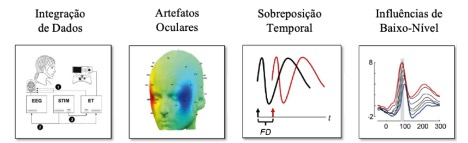
\includegraphics[width=130mm]{problemas_eeget.jpg}
    \caption[Exemplo de um acelerador linear utilizado no Hospital Universitário de Brasília.]
    {Principais problemas de integração em datasets de EEG e ET. Fonte: Dimigen e
    Ehinger (2020).}\label{fig:acelerador}
    \end{figure}


Por ser uma coleta que envolve diferentes equipamentos, a integração dos dados pode se tornar um desafio. 
Diferentes autores propuseram soluções para tal integração. A respeito do custo de equipamentos de coleta, o avanço de equipamentos comerciais tem possibilitado maior acesso à dados fisiológicos. Por exemplo, o Mindwave Mobile II (Neurosky, CA, Estados Unidos), é um exemplo de equipamento de baixo custo que captura EEG, além de também capturar outras métricas próprias do fabricante, como nível de atenção e meditação (Neurosky). O GP3 (Gazepoint, BC, Estados Unidos), por sua vez, é um equipamento comercialmente disponível que captura dados de rastreamento ocular, incluindo dilatação da pupila e direção de foco. 


    Com o propósito de desenvolver uma ferramenta de baixo custo que possa facilitar o acesso a bases de dados multimodais, o presente projeto tem por objetivo a integração dos dados coletados por estes dois equipamentos – Mindwave Mobile II e GP3. O output da ferramenta será analisado a respeito de sua capacidade de sincronização a partir dos dados de piscadas identificados em ambos os equipamentos. Acredita-se que a ferramenta proposta se apresente como uma alternativa para os equipamentos de coleta de alto custo por ser feita com equipamentos disponíveis comercialmente, e que também apresente uma oportunidade para construção de bases de dados multimodais de EEG e ET, incentivando o contínuo desenvolvimento em áreas que se beneficiem deste tipo de dataset, como BCI e diagnósticos de condições neurológicas. 


\section{Objetivos}

Criação de uma ferramenta para construção de datasets fisiológicos multimodais de EEG e ET.

\subsection{Objetivos Específicos}

\begin{itemize}
    \item Criação de um código integrativo para equipamento de coleta de EEG e ET de forma simultânea;
    \item Criação de um dataset de EEG e ET;
    \item A•	Avaliação da capacidade de sincronização dos dados multimodais pela ferramenta através da análise de sobreposição de piscadas identificadas em ambos os equipamentos;

\end{itemize}


\section{Justificativa}
AA capacidade de coletar dados fisiológicos de forma simplificada e de baixo custo pode ser um motivador para desenvolvimento de diferentes áreas em destaque na atualidade, tais como integração homem-máquina, desenvolvimento de algoritmos e automatização de processos. Outro importante fator é a diminuição da necessidade de deslocamento do participante até centros de coleta, possibilitando uma maior diversidade na população em análise (Brand et al., 2020). 

De forma geral, os benefícios da solução se concentram em:
\begin{itemize}
    \item Aumento da acessibilidade à estação de coleta, tanto por participantes quanto por pesquisadores;
    \item Aumento da volumetria de dados;
    \item Maior disponibilidade de bases de dados fisiológicos para incentivar o desenvolvimento de outras frentes de estudo;
\end{itemize}


\section{Organização do Documento}
O presente texto tem nove capítulos. 
O primeiro capítulo trata da contextualização do problema, 
objetivos gerais e específicos, e a justificativa para a abordagem selecionada. 

O segundo capítulo trata do das características da eletricidade cerebral, dando base para entendimento do que é o sinal de onda
cerebral. 

O terceiro capítulo trata do 
Rastreamento ocular, com os principais tipos de equipamento e abordagem de eletrooculograma.

O quarto capítulo aborda a acessibilidade à datasets fisiológicos e geração de bases. 

O quinto capítulo trata do uso do dataset multimodal em algortimos classificatórios.

O sexto capítulo aborda a questão da sincronização de dados de múltiplos sensores. 

O sétimo capítulo aborda os materias e métodos para construção da ferramenta e estudo de caso.

O oitavo capítulo aborda os resultados e discussões.

O nono capítulo apresenta a conclusão deste estudo. 


\chapter{Eletricidade Cerebral}



\section{Correntes Elétricas}
%Gaspar, Alberto (2005). Física:Volume único. São Paulo: Editora Ática. 496 páginas. ISBN 9788508078837. Consultado em 12 de janeiro de 2012
A eletricidade é o nome dado a uma série de fenômenos que envolvem o fluxo de cargas elétricas (Gaspar, 2005). 
O potencial elétrico (também conhecido como tensão), é a quantidade de energia precisa para deslocar uma carga elétrica (Matias e Fratezzi, 2008). 
A diferença de potencial elétrico entre um material condutor gera um fluxo de 
cargas nomeado de \textbf{corrente elétrica} (Creder, 1989).
A intensidade do fluxo é medida em ampère (A) e determinada pela quantiadade de partículas que atravessam o seguimento
do condutor pelo tempo. As correntes podem ser contínuas ou alternadas, a depender se o sentido da corrente varia ou não; enquanto a corrente contínua 
é composta de polos, a alternada é composta de fases (Bhargava e Kulshreshtha, 1983). O calculo de corrente elétrica é 
dado pela seguinte equação:

\begin{equation}
    I = \frac{\Delta Q }{\Delta T},
\end{equation}

onde $\Delta Q$ é a quantidade de particulas que passam em um seguimento do condutor e $\Delta T$ indica o tempo. 

\section{Neurônios}
Os neurônios são células responsáveis pela condução de impulsos nervosos e se comportam como um “cabo eletrificado” - analogia
levantada a respeito da condução de impulsos elétricos, como apresentado no clássico estudo de Hodgkin e Huxley (1952), 
que teve como resultado uma modelagem dos potenciais de ação emitidos pelas células 
nervosas através de equações diferenciais não-lineares (figura 2.2). 
Os neurônios comunicam-se uns com os outros através das \textbf{sinapses}, onde ocorre a transmissão dos impulsos nervosos. 
É possível distinguir três partes anatomicas no neurônio: o corpo celular, o axônio e os dendrito (figura 2.1). 

\begin{figure}
    \centering
    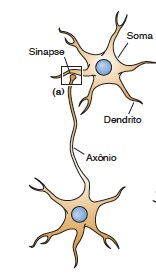
\includegraphics[width=40mm]{corpo_celular.jpg}
    \caption{Anatomia de um neurônio com destaque para área de sinapse entre neurônios. Fonte: Bear (2015)}
\end{figure}

% Serway, R.A.; Jewett Jr., J.W (2008). Princípios de Física. 3. São Paulo: Cengage Learning. p. 909-910. ISBN 85-221-0414-X
A membrana celular permite a passagem de cargas elétricas através de canais, que podem ou não necessitar de energia para a movimentação
das cargas. \textbf{Capacitores} são dispositivos de polaridades diferentes nas extremidades, que armazenam
cargas elétricas num campo elétrico (Serway, 2008). Por sua capacidade de separar cargas elétricas entre o ambiente interno e externo, 
a membrana celular age como os capacitadores, com sua capacitância (habilidade de armazenar cargas elétricas), definida pela seguinte equação:

\begin{equation}
    C = \frac{Q}{\Delta V},
\end{equation}

onde $C$ é a capacitância, $Q$ é a quantidade de carga armazenada e $\Delta V$ é a tensão elétrica, medida em farad (F). 
\textbf{Resistência elétrica} diz respeito a capacidade de oposição a passagem de corrente elétrica e é medido em
 ohms ($\Omega$). Os canais da membrana podem se comportar como resistores, se opondo a passagem da corrente elétrica, e sua 
 resistencia pode variar dependendo das condições celulares, como por exemplo se o canal está abero ou  não. Na figura 2.2, $E$ representa
 \textbf{bateria} pois a concentração de ions (particulas elétricas) é diferente no meio intra e extracelular, graças ao trabalho de canais ativos (com custo de energia
 para manter esse diferencial). De forma simplificada, a corrente aplicada no neurônio pode injetar corrente no capacitor e também 
 ser distribuída pelos canais. Dado a definição de um capacitor, $I_c = d u /d t$, é possível definir a corrente elétrica em uma seção da 
 membrana como:


%https://neuronaldynamics.epfl.ch/online/Ch2.S2.html#Ch2.F2
\begin{figure}
    \centering
    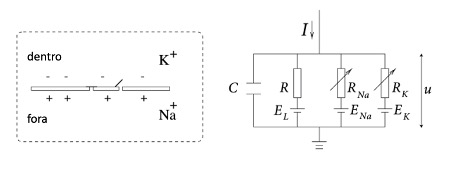
\includegraphics[width=100mm]{modeloHH.jpg}
    \caption{Esquema Modelo Hodgkin-Huxley. 
    Dentro: indicando espaço intracelular; fora: indicando espaço extracelular (imagem a esquerda). Direita: 
    C = capacitor, R = resistor, E = Baterias. Na = Sódio, K = Potássio  Fonte: Neuromal Dynamcs (2014)} 
\end{figure}

\begin{equation}
    C \frac{d u }{ d t} =  - \sum_{k} I_k (t) + I (t),
\end{equation}

onde $u$ = voltagem ao longo da membrana e $t$ = tempo. 




\subsection{Impulsos Nervosos e Potencial de Ação}
Para passar informações, os neurônios geram \textbf{impulsos nervosos}, ou alterações no potencial elétrico de sua membrana. Este sinal elétrico
ocorre quando o estímulo recebido pelo neurônio ultrapassa um limiar de ativação, que desencadeia uma série de respostas celulares. A célula pode 
estar em repouso (com valor do interior celular em cerca de -70mV), passando por despolarização (quando ocorre um fluxo de cargas elétricas que faz com 
que o meio intracelular passe a ser positivo em relação ao meio extracelular), e em repolarização, quando a célula está retornando ao potencial de repouso,
como representado na figura 2.3. 

O aumento do inicial da voltagem é causado pela entrada de sódio através de canais dependentes de voltagem, que se segue 
pela perda de potássio e fechamento dos canais de sódio. 


\begin{figure}[!h]
    \centering
    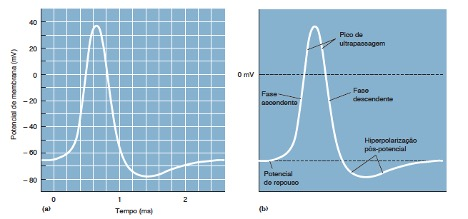
\includegraphics[width=120mm]{potencial_de_membrana_bear.jpg}
    \caption[Impulsos nervosos conduzidos em neurônios]{Resumo do potencial de ação. Fonte: Bear (2015).}.\label{fig:potencial}
    \end{figure}


\section{Eletroencefalograma}
O conjunto de impulsos nervosos de grupos de neurônios geram campos
magnéticos que podem ser captados por eletrodos colocados sobre a cabeça humana
(Kandel, 2000). Estes campos magnéticos foram primeiro registrados de coletas em
humanos aproximadamente em 1929, em um experimento conduzido pelo psiquiatra
alemão Hans Berger (Ince et al., 2021) – figura
2.4. Estes registros são o resultado dos potenciais de ação emitidos pelas células
nervosas abaixo do eletrodo, e permitem uma boa resolução temporal do
comportamento nervoso (podendo atingir precisão de milissegundos), mas em geral
não permitem uma boa resolução espacial (como identificar a localização espacial do
grupo celular responsável pela variação de voltagem observada).

  \begin{figure}[h]
    \centering
    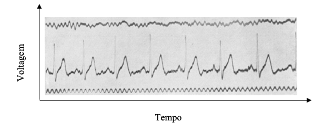
\includegraphics[width=100mm]{serie_temporal_EEG}
    \caption[]{Primeiro EEG registrado em humanos, resultado do trabalho do psiquiatra Hans Berger. Fonte: Ince et al. (2021).} 
    \end{figure}

\section{Ondas Cerebrais}
% Llinas, R. R. (2014). "Intrinsic electrical properties of mammalian neurons and CNS function: a historical perspective". Front Cell Neurosci. 8: 320. doi:10.3389/fncel.2014.00320. PMC 4219458free to read. PMID 25408634
O cérebro consegue gerar ondas ritmicas geradas pelos impulsos nervosos de grupos de neurônios. 
A oscilação de um neurônio único pode ser explorada na figura 2.3. As grandes oscilações (geradas por 
mais de um nerônio sendo ativado) pode ser detectada pelos eletrodos posicionados 
no crânio no eletroencefalograma (Llinas, 2014) e serem classificadas de acordo com suas características.
Um exemplo de agrupamento das ondas cerebrais pode ser observado na figura 2.5. 

\begin{figure}[h]
    \centering
    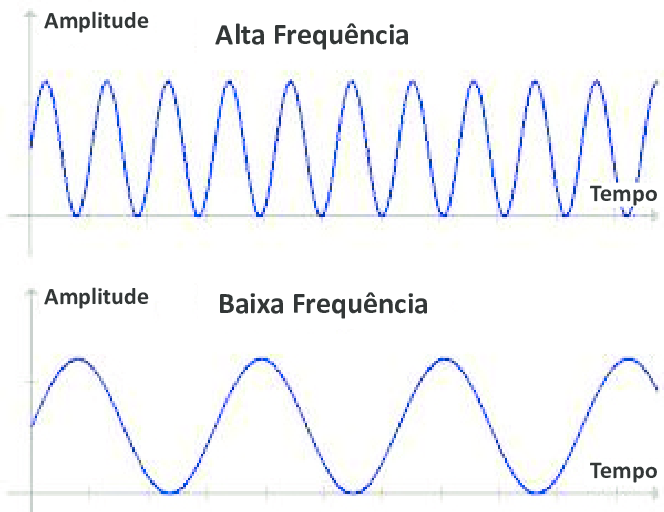
\includegraphics[width=100mm]{propriedades de onda.png}
    \caption[]{Representação das propriedades de onda.} 
    \end{figure}

As ondas cerebrais são caracterizadas pela \textbf{frequência, amplitude e fase} (figura 2.5). 
A amplitude mede a magnitude da oscilação de uma onda e pode ser representada pela equação

\begin{equation}
    y = A * sen (t - k) + b,
\end{equation}
onde $y$ é a função de onda (mede amplitude no instante t), $A$ é a amplitude da onda, sen representa
uma função senoidal, $t$ é o tempo, $k$ é a transalação temporal e b mede a translação de onda. 

\begin{figure}[h]
    \centering
    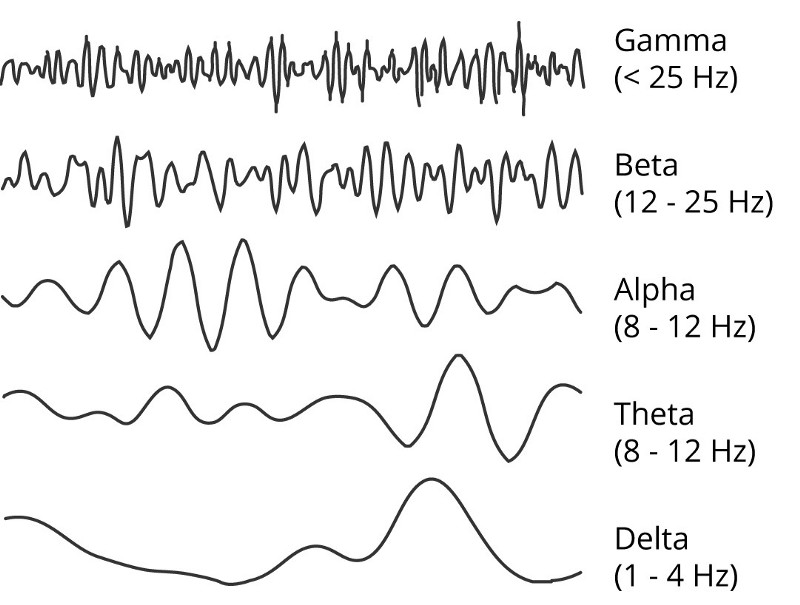
\includegraphics[width=80mm]{1_smvgacGqEOqIoKmjhzbfPw.jpeg}
    \caption[]{Ondas gamma, beta, alfa, teta e delta.} 
    \end{figure}


\subsection{Sistema Internacional 10/20 de Posicionamento de Eletrodos} 

    A técnica de registro de EEG vem sendo desde então aperfeiçoada e escolhida em
    investigações comportamentais devido a sua natureza não invasiva. Um exemplo de
    aperfeiçoamento foi a criação de um sistema internacional de posicionamentos de
    eletrodos para a coleta de EEG – o sistema 10/20 (Klem et al., 1999), 
    representado na figura 2.6.
    O registro capturado nos eletrodos
    advém de uma diferença de potencial elétrico. Esta diferença pode ser em referência à
    um eletrodo colocado em uma região externa ao escalpo (como orelha), ou à uma
    voltagem média comum (Tavares, 2011).


\begin{figure}[h]
    \centering
    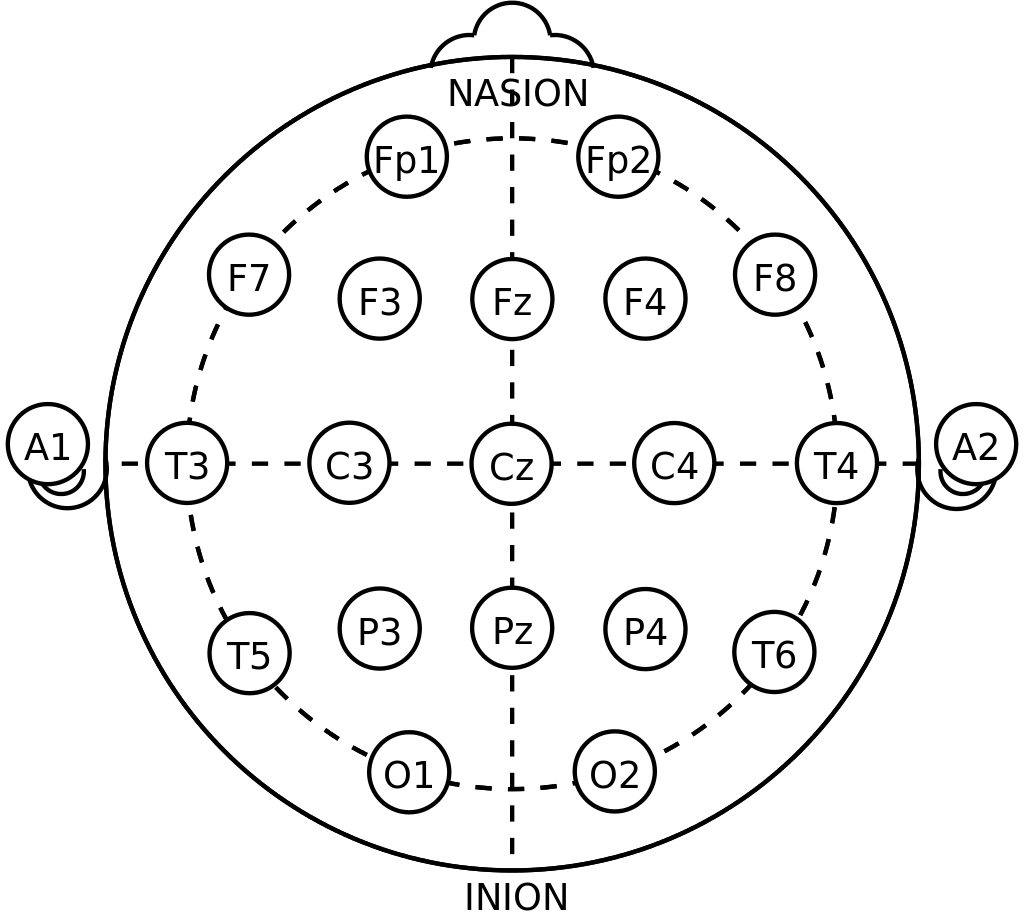
\includegraphics[width=100mm]{21_electrodes_of_International_10-20_system_for_EEG.png}
    \caption[]{Sistema Internacional 10/20 de Posicionamento de Eletrodos. Em destaque:
    Posição do eletrodo de coleta passiva do MindWave Mobile 2. A = Ear lobe, AF = anterior
    frontal, C = central, CP = centroparietal, F = frontal, FC = frontocentral, FT =
    frontotemporal, N = nasion, O = occipital, P = parietal, PO = parietooccipital, T = temporal.
    
    Klem et al. (1999).} 
    \end{figure}
    
    
        
\subsection{Tipos de Eletrodos para Captura de EEG}

    Existem diferentes tipos de eletrodos para a captura de EEG. 
    Um resumo é apresentado no quadro 2.1. É notável também que com o 
    desenvolvimento da capacidade computacional, novos recursos e métodos 
    para a análise destes dados vem sendo benéficos à construção do conhecimento 
    científico, agora também contando com o desenvolvimento de algoritmos de aprendizado
     de máquina, aprendizado profundo e inteligência artificial. 

     \begin{quadro}
        \caption{Tipos de Eletrodos para coleta de EEG (adaptado de Brain Support Inc. (2019)):}\label{quadro:exemplo}
        \begin{center}
        \scalefont{0.905}
        \begin{tabular}{|l|l|}
        \hline
        \hfill Tipo de Eletrodo\hfill\hspace{1mm} & \hfill Descrição\hfill\hspace{1mm}\\
        \hline
        Passivo &  \hspace{-06pt}\begin{tabular}{l}Geralmente feitos de prata, contam com a aplicação 
            de gel condutor \\
        para reduzir a perda de informação antes de serem colocados \\ na cabeça do participante.\end{tabular}\\
        \hline
        Ativo & \hspace{-06pt}\begin{tabular}{l}Geralmente feitos em prata, permitem o registro de \\
            variações de voltagem com redução de ruído do ambiente \\
            através de um circuito integrado aos eletrodos, com \\
            conversores de impedância.\end{tabular}\\
        \hline
        Seco & \hspace{-06pt}\begin{tabular}{l}Não necessita da aplicação de gel 
            para melhora da coleta do sinal.\end{tabular}\\
        \hline
        \end{tabular}
        \scalefont{1.4184}
        \end{center}
        \vspace{-12pt}
        Fonte: Brain Support Inc. (2019).\\
        \end{quadro}
        
  

    % Please add the following required packages to your document preamble:
% Please add the following required packages to your document preamble:
% \usepackage{graphicx}



%\subsection{Potenciais Relacionados a Eventos}




\chapter{Captura de Rastreamento Ocular}

\section{Anatomia Ocular}
O globo ocular é majoritariamente opaco, com exceção da córnea, que é transparente. 
A pupila é a região que da passagem para a luz e possui diâmetro variável. Os músculos da íris são os que controlam a dilatação da pupila. 
A focalização da imagem deve se concentrar na fóvea, onde se encontram células muito sensíveis a luz (Helene e Helene, 2011). 
A fixação ocular compreende a um período de cerca de 100 milissegundos onde o olhar se fixa em um ponto de convergência (Barreto et al., 2012). 
Este período se encerra com o movimento de sacada, que compreende ao movimento rápido até uma nova fixação do olhar em outro local.
Através da coleta do posicionamento ocular, é possível calcular uma taxa de dispersão focal ao longo do tempo e piscadas. 
Estes dados foram previamente correlacionados com estados emocionais (Soleymani et al., 2012) e 
também aplicados em estudos com algoritmos de aprendizado de máquina e deep learning. Barreto (2012)
resumiu alguns dos principais termos utilizados em pesquisas de rastreamento ocular (RO):

\section{Equipamentos de Rastreamento}
Para detectar onde o participante está focando seu olhar ao longo do tempo, alguns equipamentos de ET
 fazem uso de luz infravermelha e câmeras de alta definição que projetam a luz
  diretamente no olho do participante e gravam a direção do olhar a partir do reflexo. 
  Como a luz infravermelha abrange um comprimento de onda não detectável pelo olho humano, 
  o direcionamento desta luz no olho não interfere visão do participante. 
  O cálculo do direcionamento ocular é feito com base em algoritmos próprios de cada fabricante. 
  Existem alguns tipos de equipamentos de rastreamento ocular. São eles: (1) Webcam, (2) Vestível (Werable) e (3) Baseados em Tela. 
  Webcam diz respeito a equipamentos não especializados para o uso de rastreamento; usáveis correspondem a equipamentos como óculos de rastreamento ocular 
  e realidade virtual, e os baseados em tela dizem respeito aos equipamentos de coleta especializada que podem ser acoplados a um computador Tobii Pro (2020).

  \section{Calibração do Equipamento de Coleta}
  Como funciona a calibração

\chapter{Datasets Fisiológicos}


Apesar da existência de fontes de datasets fisiológicos públicos, 
o número de datasets disponíveis ainda é restrito. Sobre a qualidade das bases de dados, 
Mendoza et al. (2021) observou que nenhum de nove datasets disponíveis publicamente para 
treinamento de algoritmos de classificação analisados possuía 
todos os critérios de referência levantados por estudos anteriores, embora ainda mantivessem seu valor
para incentivar desenvolvimentos futuros.
Sobre a disponibilidade de datasets fisiológicos,
Rim et al. (2020) fez uma análise de datasets públicos e privados. 
No exemplo apresentado, 
é possível observar que datasets públicos combinando sinais são minoria nas diferentes fontes de dados analisadas
(figura 4.1).
\begin{figure}[!h]
      \centering
      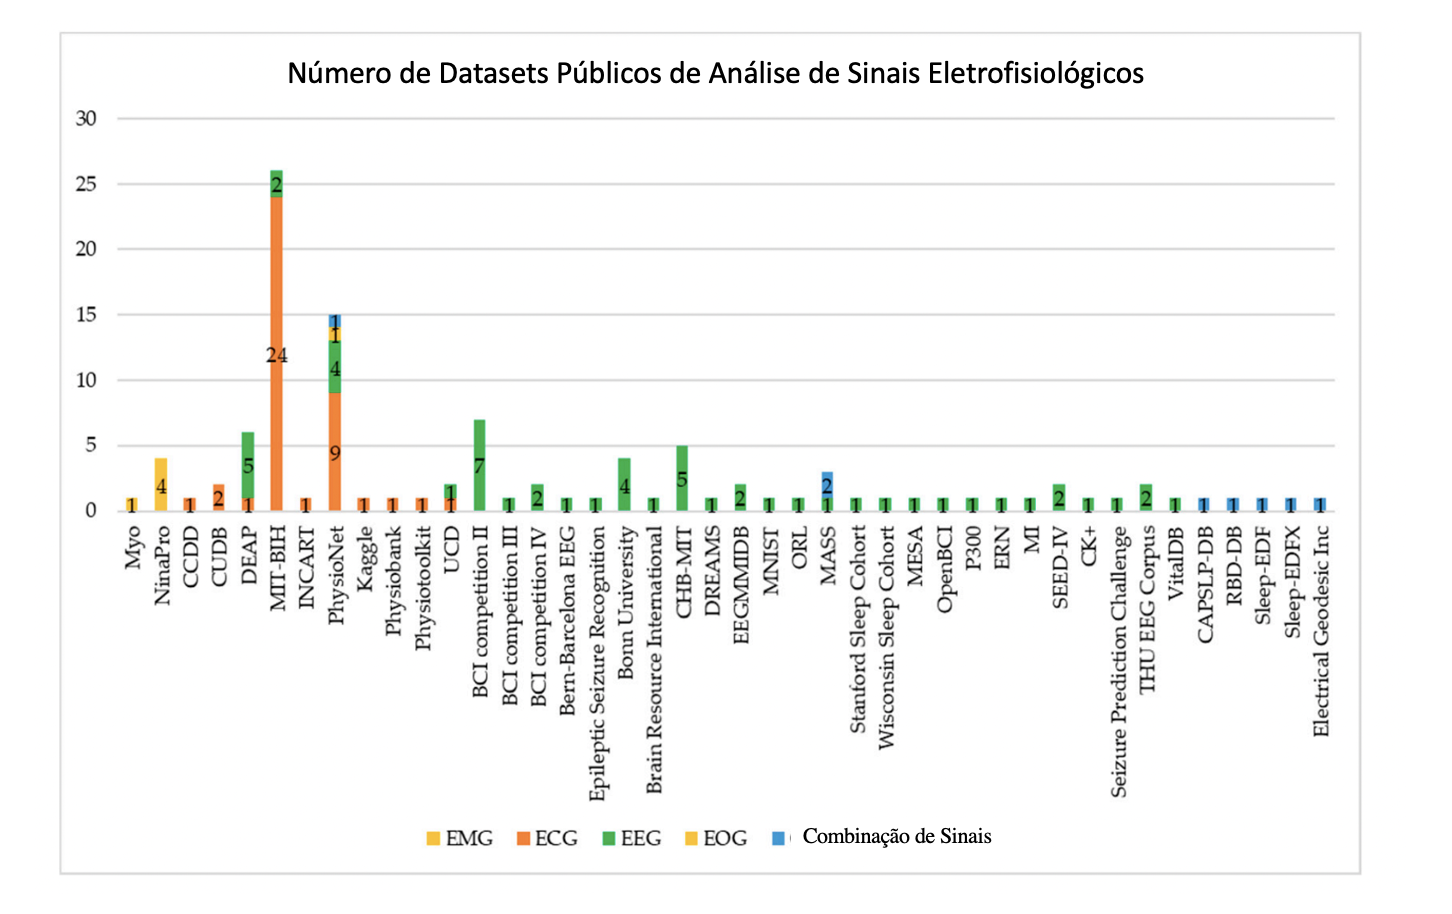
\includegraphics[width=160mm]{numero_datasets.png}
      \caption{Número de datasets disponíveis publicamente para estudos de sono por tipo de sinal. Fonte: Rim et al. (2020). }
\end{figure}

\section{Aquisição de EEG e ET}

Um exemplo de como se realizar a montagem para coleta de EEG e ET é demonstrado na figura 4.2, 
utilizado na montagem do dataset EEGEyeNet (Kastrati et al., 2021),
onde o participante é colocado de frente para o monitor para apresentação de estímulos com o 
equipamento de coleta de EEG sobre a cabeça e o aparelho de ET direcionado aos olhos. 


\begin{figure}[h]
      \centering
      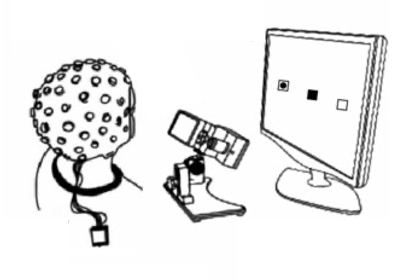
\includegraphics[width=80mm]{setup.png}
      \caption{Setup de coleta de EEG e ET. Fonte: Kastrati et al. (2021)}
\end{figure}



\section{Pré-processamento de EEG}
O pré-processamento de EEG consiste em remoção de artefatos, 
tais como contração muscular e movimentação ocular.
A etapa de extração de características consiste em, partindo dos dados com 
remoção de artefatos indesejáveis, extrair métricas estatísticas, como média, 
mediana e desvio padrão aplicados a uma janela de tempo, ou outras métricas, como entropia de Shannon 
(como feito no estudo de Thapaliya et al. (2019)). A seleção de features pode 
envolver o uso de algoritmos que permitem reduzir o número de características a 
serem apresentadas como input ao algoritmo, como o \textit{Principal Componen Analysis} (PCA).
 Um exemplo de pipeline é apresentado na figura 4.3. A partir dessas etapas, os dados são divididos entre treinamento e 
 teste, para validar o algoritmo ou algoritmos a serem estudados. 

 \begin{figure}[!h]
      \centering
      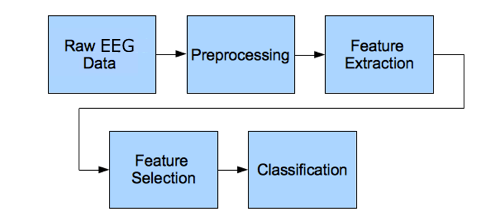
\includegraphics[width=100mm]{pipeline_eeg.png}
      \caption{Exemplo de pipeline para processamento de EEG. Fonte: Neuroeletrics (2022)}
 \end{figure}


 O pré-processamento será diferente dependendo se a fonte de dados é de \textit{single electrode} (somente um eletrodo)
 ou não, e do que é o sinal de interesse. Comumente não são estudados sinais acima de 90Hz (Neuroeletrics, 2022), 
 de forma que um filtro pode ser aplicado para remover frequencias que não forem de interesse. 
Também é comum dividir o sinal em épocas temporais de alguns segundos de duração, para extrair 
componentes destas janelas e construír a fase de extração de caractériscas. Esse processo acontece 
anteriormente a se inputar os dados a um modelo algoritmico. 

\section{A Fusão de Dados}
A fusão ou união de dados advindos de diferentes sensores pode ser realizada no nível de característica ou \textit{feature},
assim como a nível de decisão do algoritmo classificatório (Klein, 2014; Mendes et al., 2016).
      Na figura 4.4. é possível observar um fluxo de processamento dos sinais capturados por diferentes sensores.  Os diferentes 
      sensores representados no estudo de Mendes et al. (2016) são aqui representados pela coleta de EEG e ET.
 
\begin{figure}
      \centering
      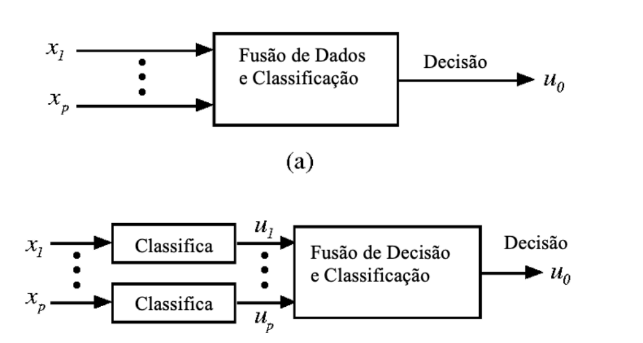
\includegraphics[width=100mm]{fusao_decisao.png}
      \caption{Exemplo de Fluxo para Fusão de Dados de Sensores. Fonte:  Mendes et al. (2016)}
\end{figure}


Na \textit{\textbf{Feature Level Fusion}} (FLF), os dados de diversas fontes são extraídos dos sensores e unidos de forma a 
gerar um vetor único com informações multimodais; no \textit{\textbf{Decision Fusion}} (DL) a classificação ocorre para cada categoria 
de fonte de dado (exemplo: uma classificação para EEG e outra para ET) e estas 
classificações são combinadas em um esquema de voto (exemplo: a classificação mais comum) 
para se chegar em uma categoria final (Bota et al., 2020). A respeito de qual formato seria melhor, 
Bota et al. (2020) observou que o melhor método de fusão é altamente correlacionado à base dados, 
embora o FLF tenha sido escolhido como o melhor em função de sua baixa complexidade em relação ao DF. 






\chapter{Uso em Algortimos}

\section{Algortimos Classificatórios}
% 

Algoritmos classificatórios
podem ser lineares ou não lineares. 
Classificadores lineares conseguem separar 
as categorias de dados em uma reta no espaço vetorial, seja ela com uma ou mais dimensões (reta, plano ou hiperplano) (Souza, 2018). Para problemas mais complexos,
é comum o uso de algoritmos que classifiquem dados não lineares, como o \textit{Support Vsector Machine} (SVM), 
\textit{K-Nearest Neightbor} (KNN) e
Rede Neural Artificial (ANN).

Para a avaliação do algoritmo, a acurácia e precisão oferecem métricas para avaliar o erro observado do output (ou resultado) do modelo. 
Para isso, é necessário saber o valor real e o valor estimado pelo algoritmo classificatório. 
A acurácia mede a proximidade de um determinado valor e o valor de referência (ou valor real) (equação 5.1). 
A precisão mede a dispersão dos valores obtidos pelo modelo (equação 5.2). Um bom algoritmo é preciso e possui alta acurácia. 

\begin{equation}
      Accuracy = \frac{TP+TN}{TP+TN+FP+FN}
\end{equation}

\begin{equation}
      Precision = \frac{TP}{TP+FP}
\end{equation}

\begin{equation}
      Recall = \frac{TP}{TP+FN}
\end{equation}

\begin{equation}
      F1 = \frac{2*Precision*Recall}{Precision+Recall} = \frac{2*TP}{2*TP+FP+FN}\text{,}
\end{equation}

onde TP = verdadeiros positivos, ou onde a previsão do valor tido com verdadeiro estava correta; TN = verdadeiros negativos;
FP e FN onde o modelo errou e em qual modalidade (se na classificação dos positivos ou dos falsos, respectivamente).
Por este motivo, existe a necessidade de separar o dataset em dataset de treino e dataset de teste. De forma habitual, o dataset
de teste é 20\% do dataset total, selecionado de forma aleatória. Ao final do momento de treinamento, onde o algoritmo 
tenta encontrar padrões nas diferentes classes do dataset, o dataset de teste é classificado pelo algortimo de acordo 
com o que foi aprendido e então as métricas de performance são calculadas. 


%referencia: Duda, Richard O.; Stork, David G. (2001). Pattern classification 2nd ed ed. New York: Wiley. OCLC 41347061
A performance de algoritmos classificatórios também pode ser observada 
através de uma matriz de confusão (Duda e Stork, 2001).
Esta matriz permite observar onde o algoritmo mais erra - se em 
classificar verdadeiros positivos ou verdadeiros negativos. 

Outra forma de avaliação é através da curva ROC, 
ou Característica de Operação do Receptor. A curva é obtida a
o se observar a variação da taxa de verdadeiros positivos 
(sensibilidade, ou Positivos Verdadeiros / Positivos Totais) em função de 1 – 
especificidade, ou taxa de falsos positivos (Positivos Falsos / Negativos Totais). 

\section{Uso de Datasets Multimodais de EEG e ET na Pesquisa}

Em seu estudo sobre o uso de algoritmos para classificação de emoções a partir de dados fisiológicos, 
Zheng et al. (2014) coletou dados de dilatação da pupila, movimentação ocular e EEG para 
identificar qual seria a classificação do estímulo emocional apresentado aos participantes. 
O processo de coleta do estudo pode ser observado na figura 5.3. 
A classificação do estímulo apresentado (vídeo clips de 4 minutos de duração) 
obteve acurácia máxima de \textbf{73.59\%} de dados coletados em 12 sessões de experimento, 
onde, em cada sessão, os 5 participantes assistiram a 15 vídeos 
(5 de emoção neutra, 5 de positiva e 5 de negativa). 
 

\begin{figure}[!h]
      \centering
      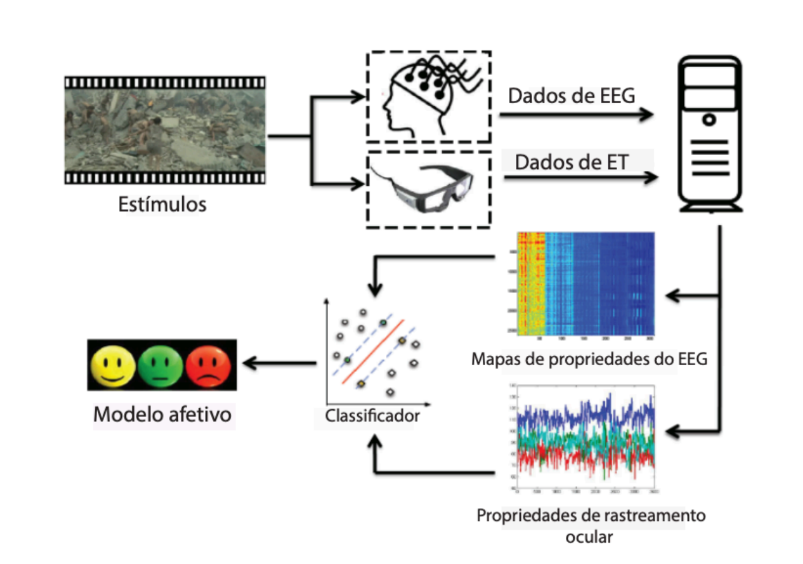
\includegraphics[width=150mm]{estimulo_e_coleta.png}
      \caption{Design de Experimento para Coleta de EEG e ET. Fonte: Zheng et al. (2014)}
\end{figure}

Lu et al. (2015) também faz uso de dados de EEG e ET para classificação de emoções nas três 
valências emocionais eleitas no estudo de Zheng et al. (2014). Em contraste com o volume de 
informações coletadas no estudo de Zheng et al., Lu et al. coletam uma maior quantidade de dados de rastreamento ocular – 
extraindo 16 métricas de ET, enquanto o estudo de Zheng foca em apenas métricas principais da dilatação ocular. 
Os resultados da acurácia do algoritmo aplicado aos diferentes métodos de fusão de dados multimodais estão resumidos na imagem 5.4, 
ficando evidente que, independente do método utilizado para fusão das modalidades de EEG e ET, 
as melhores acurácias foram encontradas para base de dados de mais de uma fonte de informação fisiológica. 

\begin{figure}
      \centering
      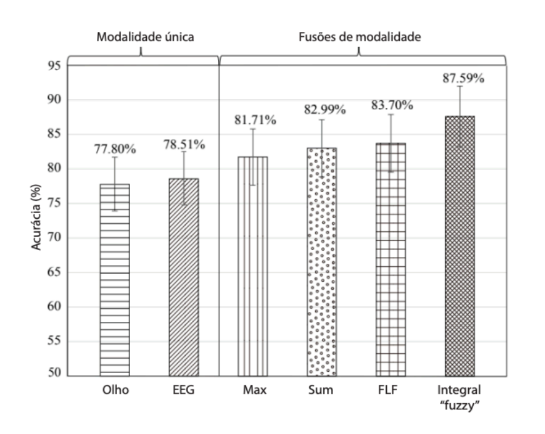
\includegraphics[width=100mm]{lu.png}
      \caption{Acurácia por Método de Fusão de Modalidade e Modalidade Única em Algoritmo Supervisionado. Fonte: Lu et. al. (2015)}
\end{figure}

No trabalho de Thapaliya et al. (2019) dados de EEG e ET foram aplicados em algoritmos de máquina, 
com o objetivo de estudar uma melhora no método de diagnóstico de crianças com autismo através de 
diferentes formas de pré-processamento (exemplo de processamento do estudo na figura 5.5). 
Os dados de EEG tiveram suas métricas estatísticas coletadas para a construção de um vetor de características 
(incluindo desvio padrão e média por janela de tempo dos dados de EEG filtrados), assim como a entropia calculada 
por janela temporal. Para os dados de ET, os tempos de fixação foram coletados, em conjunto com o resultado de testes cognitivos. 
Em seu estudo, diferentes métodos de construção de vetores de características foram analisados, 
tanto para os dados unimodais quanto para a junção de EEG e ET. 
Através das acurácias apresentadas para os diferentes métodos de processamento, 
é possível observar que determinados algoritmos aumentaram sua acurácia a
 depender do modo no qual o vetor de características foi construído. 
 Por exemplo, enquanto o algoritmo Support Vector Machine (SVM) atingiu \textbf{71\%} de acurácia 
 com o vetor que incluiu Entropia para as janelas de EEG e PCA, a regressão logística com maior acurácia 
 foi atingida com o dataset de desvio padrão de EEG e dados de rastreamento ocular sem a aplicação de PCA 
 (Thapaliya et al., 2019). 

Lim e Chia (2015), estudaram a correlação de ondas EEG detectadas em um equipamento de eletrodo único e 
estresse cognitivo induzido pelo teste de Stroop. A análise foi feita com base na aplicação de três algoritmos: 
\textit{Artificial Neural Network}, \textit{k-Nearest Neighboor} (KNN) e \textit{Linear Discriminant Analysis} (LDA), 
dos dados de EEG transformados pela aplicação da Transformação Cosseno Discreta (\textit{Discrete Cosine Transform} – DCT). 
O KNN com o DCT conseguiu classificar melhor o estado de estresse do participante.

\section{Equipamentos Comerciais na Pesquisa}

O uso do MindWave Mobile II foi recentemente empregado para o 
controle de cadeira de rodas (Abuzaher e Al-Azzeh, 2021; Permana et al., 2019), 
controle de mão robótica e robô móvel (Purnamasari et al., 2019; Rusanu et al., 2019; Rușanu et al., 2021) 
e predição de personalidade (Bhardwaj et al., 2021). 

Outro estudo com uso de eletrodo único como fonte de dados eletrofisiológicos foi o trabalho de Quesada-Tabares et al. (2017), 
onde foi demonstrado que o uso de EEG comercial e com eletrodo único também possui um importante poder classificatório 
quando aplicado em algoritmos. Em seu estudo, sete participantes observaram imagens selecionadas do 
\textit{International Affective Picture System} (IAPS) pertencentes a três grupos com diferentes valores de 
valência e excitabilidade. O teste de Análise de Variância aplicado indicou 
uma diferença estatisticamente significante entre os sets de imagens.
 Um segundo teste foi conduzido pela aplicação de um algoritmo de classificação no estilo árvore de decisão,
  chegando a uma acurácia média entre os sete participantes de \textbf{80.71\%}.

Bos (2021) também explora o uso do Mindwave no contexto escolar para medir a atenção dos alunos. Em seu estudo, 
o nível de atenção com alunos assistindo a um vídeo educacional sem e outro com interações (fazendo pergunta aos alunos)
 é explorado e a distribuição percentual das diferentes bandas de frequência são comparadas entre os grupos. Foi 
 observado uma relativa diminuição banda de frequência de onda beta para o grupo que não assistiu ao vídeo interativo, 
 o que foi relacionado a um processamento cognitivo reduzido e menor atenção.


%Bhardwaj et al. (2021) analisou o uso dos dados coletados com o Mindwave para classificar sete traços de personalidade 
%com o algoritmo \textit{deep long short term memory} (DeepLSTM) e tratando os dados com transformada de Fourier Rápida. 
%A pesquisa contou com 50 participantes (25 mulheres e 25 homens), com idades entre 18 e 46 anos, e durou cinco dias.
%Os dados foram coletados enquanto os participantes assistiam vídeos relacionados a traços de personalidade. 
% Os traços foram separados de acordo com os tipos de personalidade definidos no \textit{Myers-Briggs Type Indicator}, 
% e ao final de cada vídeo, o participante deveria dizer se concordava, 
% discordava ou era neutro aos questionários de personalidade sobre o traço proeminente no estímulo. 
% O questionário de cada participante foi utilizado para determinar o traço de personalidade, 
% que serviria para então classificar os dados em três possíveis outputs: 
% (a) participante tem traço de personalidade apresentado no vídeo, (b) participante não tem traço apresentado de forma significativa 
% e (c) participante tem traço oposto ao apresentado no vídeo.
 
% [FALTOU CONCLUSÃO AQUI]


\begin{figure}[h]
      \centering
      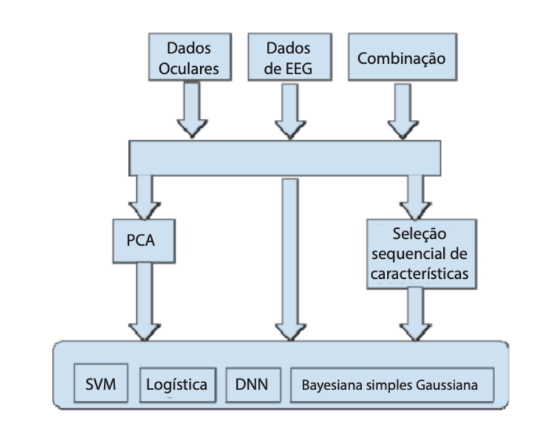
\includegraphics[width=100mm]{thapalya.png}
      \caption{União de dados de EEG e ET. Fonte: Thapaliya et al. (2019)}
\end{figure}

\section{Considerações Finais}
Datasets multimodais tendem a performar melhor em algoritmos classificatórios que datasets unimodais. 
A forma de processamento dos dados também pode ter impactos na performance classificatórias dos algoritmos. 
Equipamentos comerciais já foram previamente utilizados em estudos de algoritmos classificatórios. 
É esperado que um método de tratamento eficiente reflita em uma maior acurácia dos algoritmos treinados no dataset. 



\chapter{Sincronização}

O uso de equipamentos com função exclusiva de sincronização para coletas simultâneas é comum em pesquisas ambientes academicos e clínicos.
A proposta de oferecer maior acessibilidade através da redução de custo e desenvolvimento de novas tecnologias encontra, portanto, um desafio a respeito 
de como realizar a sincronização dos dados fisiológicos sem abrir mão da praticidade e custo dos equiapementos desenvolvidos. 
Algumas propostas já foram exploradas a respeito, como o uso de piscadas e código temporal para garantir a sincronização de EEG e ET (Bækgaard et al. 2015, Notaro et al. 2018).

\section{Frequência de Coleta}
Como os sinais análogos são convertidos para sinais digitais, existe uma perda de informação por esta conversão. 
A \textbf{resolução de frequência} mede o espaço entre duas frequências. 

$$srate/N$$

Srate = sampling rate 
N = Número de amostras

\subsection{Frequência Nyquist}
É a frequência mais rápida onde o sinal pode ser medido, onde é estabelecido que a maior frequência que podemos medir é a metade 
da frequência de coleta.s


\section{Sincronização com Timecode}
Notaro et al. (2018) faz uso do código temporal, ou \textit{timecode}, para sincronizar dados de EEG, ET e dados comportamentais 
coletados de participantes enquanto estes faziam atividades de um site de aprendizagem de linguas. O driver
do fabricante do equipamento comercial de EEG utilizado permite alteração da latência da coleta de dados, que
foi modificada do valor padrão de 16 milissegundos para 1 millisegundo, afim de aumentar a precisão do equipamento.
A informação da ocorrência de clicks no site foi retina na forma de milissegundos (HH:MM:SS:MsMsMs), e esta informação foi utilizada 
para sincronizar dados de ET, EEG e movimentação de mouse. 

\section{Sincronização com Piscadas}
Piscadas duram cerca de 200 milissegundos em média e podem indicar estados de alerta (Caffier, 2013). Piscadas também aparecem 
em dados de EEG de forma característica, podendo alcançar uma amplitude de sinal acima de 200 microvolts em eletrodos próximos a órbita ocular (Hoffmann e Falkenstein, 2008). Assim sendo, é possível realizar uma sincronização por piscadas ao se detectar 
o movimento em ambos os equiapmentos de coleta. No caso do EEG, as piscadas são comumente descartadas como artefatos indesejáveis. Já no estudo de 
Bækgaard et al. (2015), elas são a assinatura de sincronização entre os equipamentos de coleta de EEG e ET em função de sua onda característica (geralmente muitos milivolts acima do sinal do EEG), e de também 
ser detectdo através dos equipamentos de rastreamento ocular.

O desafio da sincronização de EEG e ET se dá em função de serem séries temporais muito distintas e 
de frequências de amostra diferentes. No caso dos equipamentos comerciais de interesse desta pesquisa,
a coleta de EEG pode ser realizada em até 512 Hz, enquanto a frequencia de coleta de ET chega num máximo de 60 Hz. 
Além disso, o sinal de EEG pode apresentar mais de um canal, enquanto dados de ET podem ser representados
na forma de coordenadas. Desta forma, Bækgaard et al. (2015) propõe uma sincronização por assinaturas dentro de cada um dos tipos de dados
coletados. Piscadas ocorrem com frequencia e de forma expontanea, além de ser uma informação capturada em 
equipamentos de EEG e ET.




\subsection{Identificação no Sinal do EEG}

A piscada envolve ativação muscular, e o dipolo ocular também influencia na captura de alterações de voltagem em eletrodos próximos aos olhos
(Croft e Barry, 2000). Seu reflexo no EEG pode ser facilmente identificado pois tente a ter uma amplitude e forma de sinal característicos. 
A amplitude de uma atividade de piscada no sinal de EEG tem uma média de 200 microvolts (Hoffmann et al., 2008). Esta característica permite
que o poder elétrico somado de eletrodos de interesse possam auxiliar na determinação de uma probabilidade do evento capturado ser uma piscada. 
No estudo de Bækgaard et al. (2015), as assinaturas de piscadas foram alinhadas entre as modalidades de EEG e ET para garantir a sincronizaçã, e
o começo da atividade de piscada (com o fechamento das pálpebras) foi eleito como o ponto de referencia da assinatura. 


Para se detectar a piscada através de um sinal, é possível tentar realizar o método de \textit{Independent Component Analysis}, ou análise de 
componente independente, mas as características do sinal de piscada também permite outras abordagens, como a identificação por função de probabilidade.


\subsection{Identificação no Sinal de ET}
Como o equipamento de rastreamento procura encontrar sinais da movimentação ocular, ele também detecta a ausencia desse sinal. No estudo 
de Bækgaard et al. (2015), uma perda de até 500 milissegundos foi considerada como indicador da ocorrência de uma piscada. No equipamento de coleta de ET GP3, 
o fabricante oferece uma forma de identificar a existencia de uma piscada. Ela ocorre através da propriedade Blinking Validation Flag, ou BKID, onde qualquer 
valor diferente de 0 indica ocorrência de piscada durante o timeframe. A extração de piscada através do BKID foi utilizada no estudo de Seha et al. (2019), 
onde o blink rate foi validado e sincronizado com o vídeo do próprio equipamento (que indica quando houve piscada através da ausencia da imgem dos olhos do usuário).

\section{Correlação Cruzada}
A correlação cruzada procura calcular a similaridade entre dois sinais com a aplicação de um \textit{delay} em apenas um dos sinais.
Com dois sinais diferentes em EEG e ET, Bækgaard et al. (2015) opta por correlacionar as funções de probabilidade do evento observado em 
ambos os equipamentos, ser uma piscada. 
Para correlacionar assinaturas diferentes, as probabilidades de ocorrencia de um evento (piscada) em duas séries temporais são convertidas em uma mesma frequência amostral (Bækgaard et al., 2014).
A similatidade entre sinais é medida na amplitude do sinal da correlação. A correlação cruzada é definida como:
\begin{equation}\label{eq:correlação cruzada}
    (f * g) = f(-t)*g(t), 
    \end{equation}
onde * significa convolução e f(-t) é o conjugado complexo de f(t).


\section{Códigos para Sincronização}
Alguns equipamentos podem se beneficiar da existencia de \textit{toolboxes} ou bibliotecas direcionadas à sincronização. É o caso 
dos equipamentos Tobii na solução de EEG-Eye para a linguagem MATLAB. Uma forma de se fazer sincdronização é através 

\section{Correlação EEG e ET}

 Shared triggers
Common trigger pulses ("triggers") are sent frequently from the 
stimulation computer to both ET computer and EEG recording computer. 
This is achieved via a Y-shaped cable that is attached to the parallel 
port of the stimulation computer and splits up the pulse so it is looped through 
to EEG and ET. We recommend to send triggers with a sufficient duration 
(e.g. at least 5 ms at 500 Hz sampling rate) to avoid the loss of some of the triggers.
 The advantage of this method is that the same physical signal is used for 
 synchronization (although this does not guarantee that the trigger is
  inserted into the ET and EEG data streams without delays). The disadvantage
   is the need for an extra cable.

Messages+triggers
Messages are short text strings that can be inserted into the eye tracking data.
 While triggers are still sent to the EEG, messages are used as the corresponding 
 events for the ET. Here, the ET computer is given a command to insert an ASCII text 
 message (containing a keyword and the value of the corresponding EEG trigger) 
 into the eye tracking data. In the stimulation software, the commands to send a trigger
  (to the EEG) and a message (to the ET) are given in immediate succession. 

  Analogue output
  A copy of the eye track is fed directly into the EEG. A digital-to-analogue 
  converter card in the ET outputs (some of) the data as an analogue signal.
   With SMI, this signal can be fed directly into the EEG headbox. 
   This requires a custom cable and resistors to scale the output voltage 
   of the D/A converter to the EEG amplifier's recording range. While this
    method affords easy synchronisation, there are disadvantages: First, 
    voltages need to be rescaled to pixels for analysis. Second, the ET 
    signal may exceed the amplifier’s recording range and electrical 
    interference with the EEG is possible. 
    Third, additional information from the ET 
    (messages, eye movements detected online) is 
    not available. Fourth, quality of the ET signal 
    suffers considerably from the D/A and subsequent 
    A/D conversion. Finally, fewer channels remain to record
     the EEG (recording binocular gaze position and pupil diameter occupies six channels).

     Basics: Synchronization signals

     Send triggers and/or messages to align the recordings
The toolbox requires that there are at least two shared events present in the ET and EEG: One near the beginning and one near the end of the recording. These events will be called start-event and end-event in the following. Eye tracking data in between the start-event and end-event will be linearly interpolated to match the sampling frequency of the EEG. We recommend to use a unique event value (e.g. "100") to mark the start-event and another unique event-value (e.g., "200") for the end-event. The remaining shared events (triggers or messages) sent during the experiment (between start-event and end-event) are used to evaluate the quality of synchronization. Synchronization is possible even if some intermediate events were lost during transmission.

Original sampling rates of EEG and ET do not need to be the same. The ET will be resampled to the sampling frequency of the EEG. For example, if the EEG was sampled at 500 Hz, and eye movements were recorded at 1000 Hz, the toolbox will downsample the eye track to 500 Hz. Since ET data outside of the synchronization range (before start-event, after end-event) cannot be interpolated, it is replaced by zeros. Please note that the EEG recording should not be paused during the experiment. [Clarification, April 2013: It is not a problem to pause the eye tracker recording, e.g. for recalibrations, because the time stamp assigned to each ET sample continues to increase even during the pause. However, the toolbox currently cannot recognize and handle pauses in the EEG recording. Therefore, the EEG recording should be continuous and must not be paused.]

Note:The current Beta version of the toolbox does not yet implement low-pass filtering of the eye track to prevent aliasing in case that the eye track is downsampled to a much lower EEG sampling rate. We plan to add this in the future.

If synchronization method 2 (messages plus trigger) is used, synchronization messages sent to the eye tracker need to have a specified format. This format consists of an arbitrary user-defined keyword (e.g., "MYKEYWORD") followed by an integer value ("MYKEYWORD 100"). The integer value needs to be the same as that of the corresponding trigger pulse sent to the EEG (usually an 8-bit number between 1 and 255). An example is given in the code below. The EYE-EEG parser (Step 2: Preprocess eye track and store as MATLAB) will recognize messages with the keyword and treat them as synchronization events. A keyword-synchronization messages should be sent together with every trigger sent to the EEG, so intermediate events in-between start-event and end-event can be used to assses synchronization quality. Additional messages (that do not contain the keyword) may be sent to code other aspects of the experimental design. They are ignored by the toolbox.

The following code is an example for an experimental runtime file containing the necessary synchronization signals. The example is for the software Presentation™, but similar commands exist in other software (e.g., Psychtoolbox, EPrime™):

%\chapter{Algortimos de Classificação}

A variável de interesse no aprendizado de máquina pode ser categórica, também chamada de qualitativa. 
No aprendizado supervisionado, o dataset previamente classificado é normalmente dividido entre
dataset de treinamento e teste. Esta divisão permite que a avaliação do algoritmo seja feita em dados 
não utilizados anteriormente, evitando um viés durante a avaliação do poder classificartório. Existem 
diferentes métodos de classificação em aprendizado de máquina. Alguns dos principais métodos
serão apresentados a seguir.

\section{Regressão Logística}
A regressão logistica utiliza uma função de ativação para determinar a probabilidade 
das características do dataset serem representantes de uma dada categoria e todas as 
probabilidades ficam entre valores de zero ou um (equação 7.1).

\begin{equation}
      p(X) = \beta_{0} + \beta_{1}X,
\end{equation}
onde $p(X)$ é a probabilidade da categoria. Para que o valor da probabilidade 
permaneça entre 0 e 1, a função logística é utilizada (equação 7.2).

\begin{equation}
      p(X) = \frac{e^{\beta_{0} + \beta_{1}X}}{1 + e^{\beta_{0} + \beta_{1}X}},
\end{equation}
onde a probabilidade resultante sempre estará entre 0 e 1. 





\section{Avaliação de Algoritmos Classificatórios}

A acurácia e precisão oferecem métricas para avaliar o erro observado do output (ou resultado) do modelo. 
Para isso, é necessário saber o valor real e o valor estimado pelo algoritmo classificatório. 
A acurácia mede a proximidade de um determinado valor e o valor de referência (ou valor real) (equação 7.1). 
A precisão mede a dispersão dos valores obtidos pelo modelo (equação 7.2). 
Um bom algoritmo é preciso e possui alta acurácia. 

\begin{equation}
      Accuracy = \frac{TP+TN}{TP+TN+FP+FN}
\end{equation}

\begin{equation}
      Precision = \frac{TP}{TP+FP}
\end{equation}

\begin{equation}
      Recall = \frac{TP}{TP+FN}
\end{equation}

\begin{equation}
      F1 = \frac{2*Precision*Recall}{Precision+Recall} = \frac{2*TP}{2*TP+FP+FN}\text{,}
\end{equation}

onde TP = verdadeiros positivos, ou onde a previsão do valor tido com verdadeiro estava correta; TN = verdadeiros negativos;
FP e FN onde o modelo errou e em qual modalidade (se na classificação dos positivos ou dos falsos, respectivamente).
Por este motivo, existe a necessidade de separar o dataset em dataset de treino e dataset de teste. De forma habitual, o dataset
de teste é 20\% do dataset total, selecionado de forma aleatória. Ao final do momento de treinamento, onde o algoritmo 
tenta encontrar padrões nas diferentes classes do dataset, o dataset de teste é classificado pelo algortimo de acordo 
com o que foi aprendido e então as métricas de performance são calculadas.




\include{fundamentacao_teorica/chap_materiais_e_métodos.tex}

\chapter{Resultados}
O dataset de EEG e ET foi construído com uma frequência de 60 Hz. Cada linha 
temporal contendo informação de dados de movimentação ocular e dados de EEG sem pré-processamento. 

\section{Construção do Dataset}
Dados de baixa qualidade são removidos. Estes consideram a coluna identificadora de má qualidade 
do aparelho GP3, e a ausencia de alteração por longos períodos (1 segundo) do raw EEG. 

\section{Sincronização}






\chapter{Discussão}\label{chap:Discussao}
Durante a análise de performance do equipamento GP3, a métrica USER 
foi utilizada por Brand et al. (2020) para identificar o estímulo apresentando
no dado timecode e também a captura de clicks no mouse. Segundo o fabricante, 
a coluna USER é utilizada para que o usuário possa enviar mensagens ao equipamento. 
O Código que gera os dados multimodais utiliza da mesma via disponibilizada pelo 
fabricante do equipamento para indicação de estímulos apresentados. Entretanto,
ao invés da identificação de estímulo apresentado, o código captura o dado de EEG 
no determinado momento, possibilitando que o dataset gerado tenha informações de ambos, EEG e ET, 
para cada momento de coleta. Como no estudo apresentado sobre a qualidade dos dados do GP3, realizado por Brand et al. (2020),
a coleta com a ferramenta multimodal também deverá considerar os principais fatores que impedem uma coleta de 
qualidade, sendo estes: distancia do equipamento, reflexos no olho e calibração adequada. 

O código possibilitou a geração de um datasetmultimodal coletado em um reduzido espaço de tempo. 
Para atestar a sincronização dos equipamentos, a presença de curvas típicas de piscadas foram 
identificadas em conjunto com a identificação de piscadas pelo equipamento GP3. Além da calibração
realizada desta forma, 

\chapter{Conclusão}\label{chap:Conclusao}

\renewcommand\bibname{\Large\scshape Lista de Referências}
\addcontentsline{toc}{chapter}{\bf Lista de Referências}
\bibliography{referencias}

% |--- Exemplos de Apêndices ---|----------------------{{{
% Início do Apêndice
\newcounter{apendice}
\counterwithin{figure}{apendice}
\counterwithin{table}{apendice}
\renewcommand{\theapendice}{\Alph{apendice}}
\DeclareRobustCommand{\novoapendice}[1]{%
    \refstepcounter{apendice}%
    \phantom{\theapendice}\label{#1}}

% Exemplo 1
\clearpage
\begin{flushright}
\novoapendice{apendice_exemplo}
\scalebox{1.3}{\bfseries\scshape Apêndice~\ref{apendice_exemplo}}
\addcontentsline{toc}{chapter}{Apêndice~\ref{apendice_exemplo}}
\end{flushright}

\noindent\begin{large}{\bfseries\scshape Exemplo de Apêndice}\end{large} \label{sec:apendice1}

\vspace{24pt}

Se você desejar, pode incluir ao final um ou mais apêndices, e um ou mais anexos. Caso não queira, é só remover todo o conteúdo começando na linha marcada por ``\%~Início~do~Apêndice'', até a linha anterior a ``\verb|\end{document}|''.

% Exemplo 2
\clearpage
\begin{flushright}
\novoapendice{apendice_outro_exemplo}
\scalebox{1.3}{\bfseries\scshape Apêndice~\ref{apendice_outro_exemplo}}
\addcontentsline{toc}{chapter}{Apêndice~\ref{apendice_outro_exemplo}}
\end{flushright}

\noindent\begin{large}{\bfseries\scshape Outro Exemplo de Apêndice}\end{large} \label{sec:apendice2}

\vspace{24pt}

Se você desejar, pode incluir ao final um ou mais apêndices, e um ou mais anexos. Caso não queira, é só remover todo o conteúdo começando na linha marcada por ``\%~Início~do~Apêndice'', até a linha anterior a ``\verb|\end{document}|''.
%---}}}

% |--- Exemplos de Anexos ---|----------------------{{{
% Início do anexos
\newcounter{anexo}
\counterwithin{figure}{anexo}
\counterwithin{table}{anexo}
\renewcommand{\theanexo}{\Alph{anexo}}
\DeclareRobustCommand{\novoanexo}[1]{%
    \refstepcounter{anexo}%
    \phantom{\theanexo}\label{#1}}

% Exemplo 1
\clearpage
\begin{flushright}
\novoanexo{anexo_exemplo}
\scalebox{1.3}{\bfseries\scshape Anexo~\ref{anexo_exemplo}}
\addcontentsline{toc}{chapter}{Anexo~\ref{anexo_exemplo}}
\end{flushright}

\noindent\begin{large}{\bfseries\scshape Exemplo de Anexo}\end{large} \label{sec:anexo1}

\vspace{24pt}

Se você desejar, pode incluir ao final um ou mais apêndices, e um ou mais anexos. Caso não queira, é só remover todo o conteúdo começando na linha marcada por ``\%~Início~do~Apêndice'', até a linha anterior a ``\verb|\end{document}|''.

% Exemplo 2
\clearpage
\begin{flushright}
\novoanexo{anexo_outro_exemplo}
\scalebox{1.3}{\bfseries\scshape Anexo~\ref{anexo_outro_exemplo}}
\addcontentsline{toc}{chapter}{Anexo~\ref{anexo_outro_exemplo}}
\end{flushright}

\noindent\begin{large}{\bfseries\scshape Outro Exemplo de Anexo}\end{large} \label{sec:anexo2}

\vspace{24pt}

Se você desejar, pode incluir ao final um ou mais apêndices, e um ou mais anexos. Caso não queira, é só remover todo o conteúdo começando na linha marcada por ``\%~Início~do~Apêndice'', até a linha anterior a ``\verb|\end{document}|''.
%---}}}

\end{document} 
%---}}}
